\paragraph{Entity relationship diagram}
\mbox{}\par

The ERD has 11 entities, grouped into accounts, friendships, conversations and
messages, spam reports, and sign-ins and activity. \texttt{Conversation} is shared
by private conversations and group chats, told apart by the \texttt{type}
attribute. Members and their rights in each conversation are managed through
\texttt{ConversationMember}.

Figure~\ref{fig:erd-chatapp-v1} shows the whole model. The attributes are
described again in Table~\ref{tab:data-dictionary} for easy reference.
In the figure, PK is a primary key, FK a foreign key and UK a unique value;
a question mark marks an attribute that may have no value. The symbols 1 and 0..N
show a one-to-many relationship, where the many side may have no records yet.

\begin{landscape}
\begin{figure}[p]
  \centering
  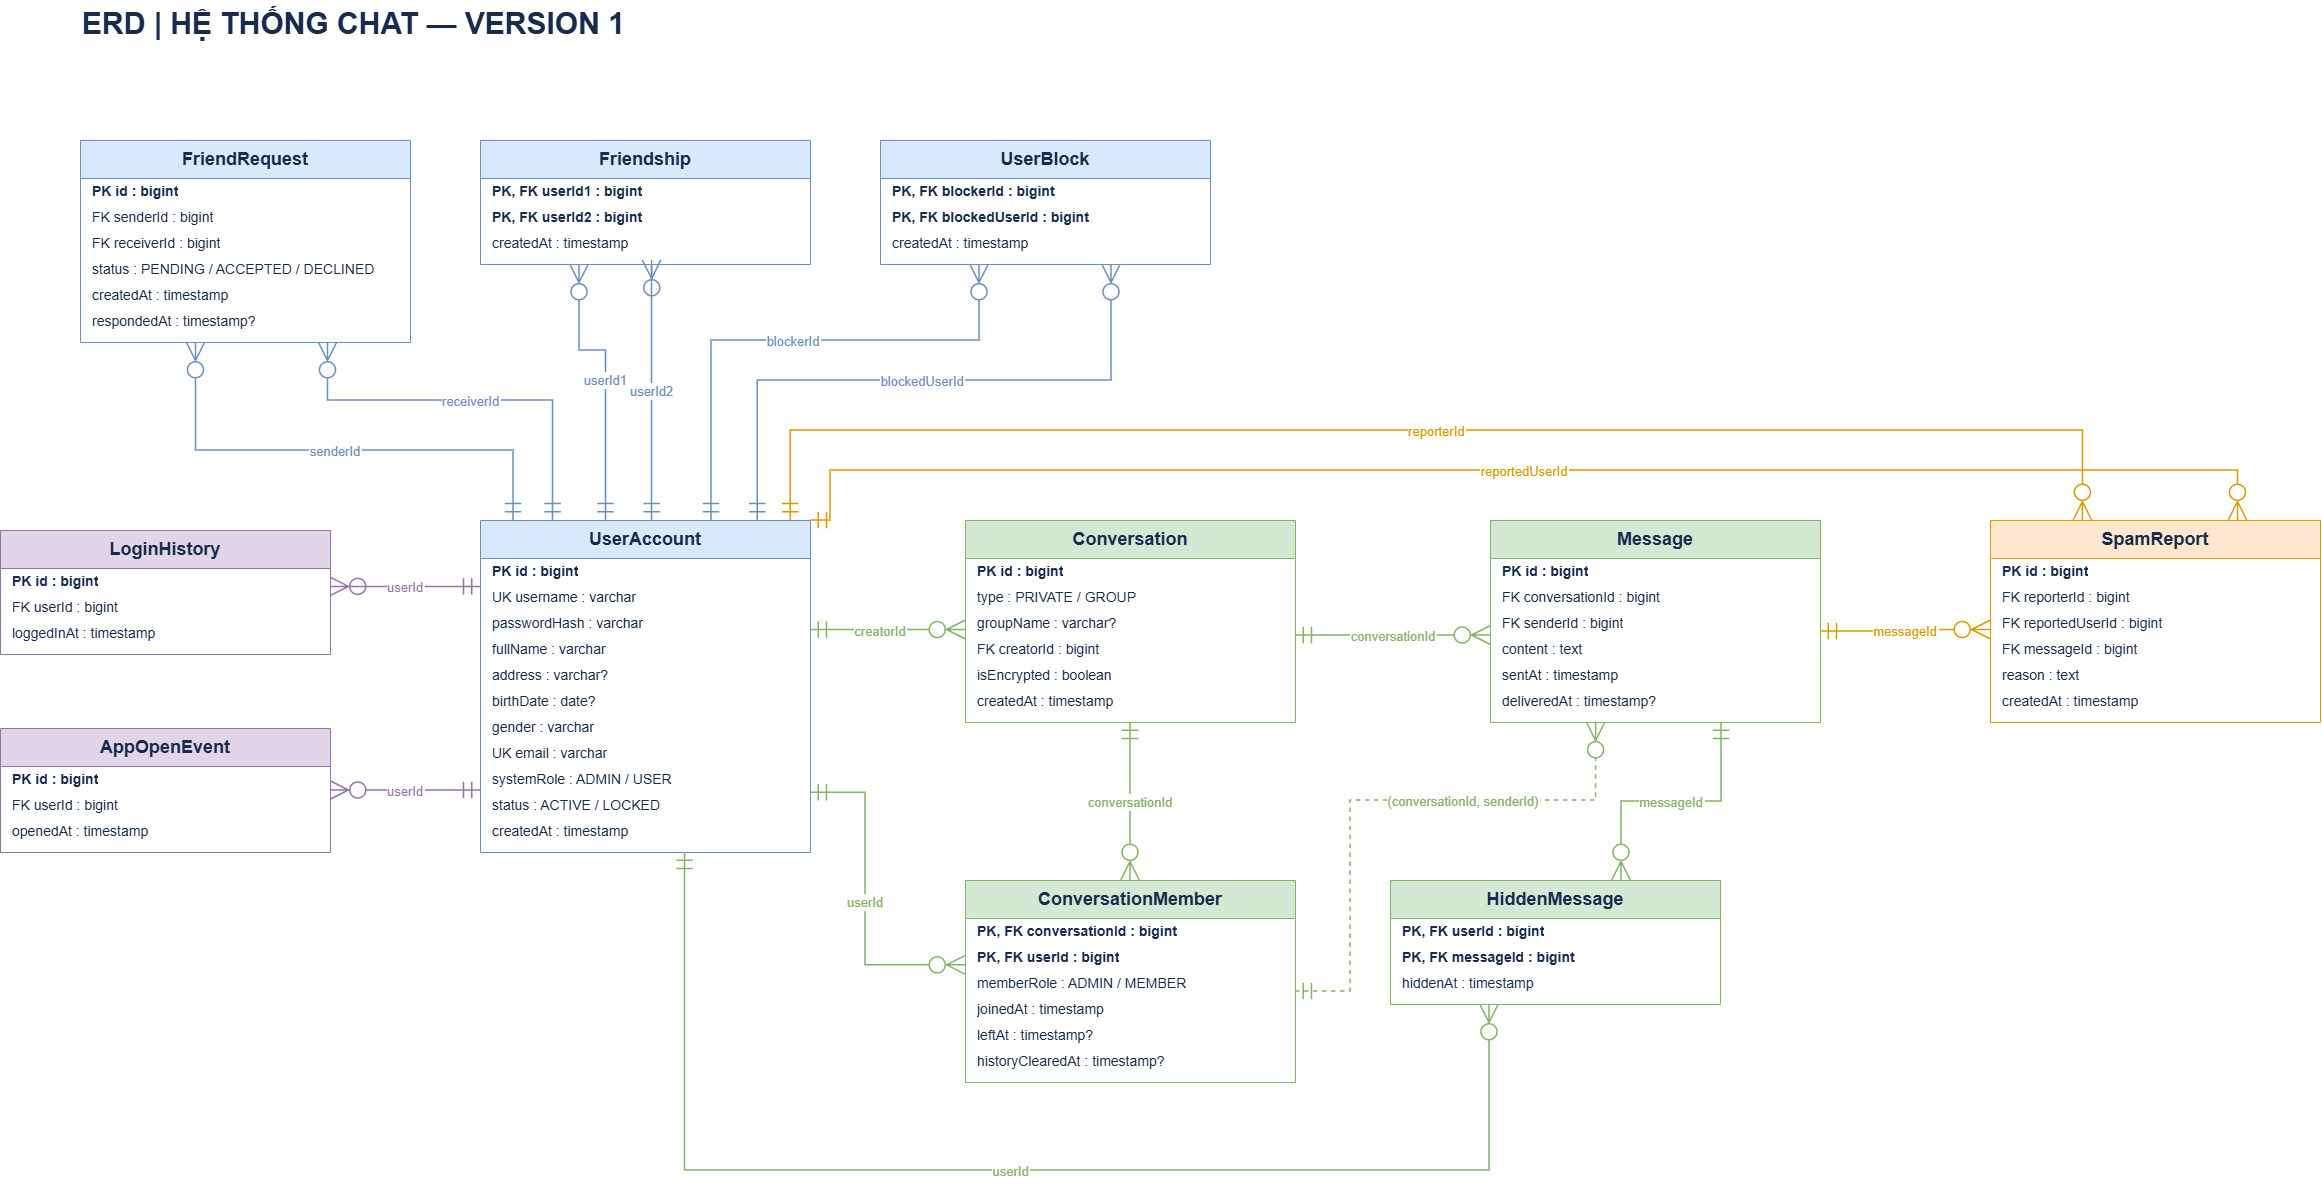
\includegraphics[width=\linewidth,height=0.83\textheight,keepaspectratio]{images/ERD-chatapp-v1.drawio.png}
  \caption{Entity relationship diagram of the chat system.}
  \label{fig:erd-chatapp-v1}
\end{figure}
\end{landscape}

Entity and attribute names in the text match the diagram. Data types in the ERD
are logical; string lengths, default values and the on-delete policy are decided
when the PostgreSQL script is finished.
